\documentclass[Main.tex]{subfiles} 
\begin{document}

\section{Experiment - Anchoring}

In this experiment for the prototype session we try to affect the results of the session by anchoring the participants. As described in the theory section anchoring (\ref{anchor}), the participants are required to fill out a questionnaire in which they state how much they like each of the new features (on a scale 1 to 10) that are mentioned along with some more general questions lead-in questions. The questions display the averages of a 'hypothetical' prior experiment.  \\

\begin{figure}
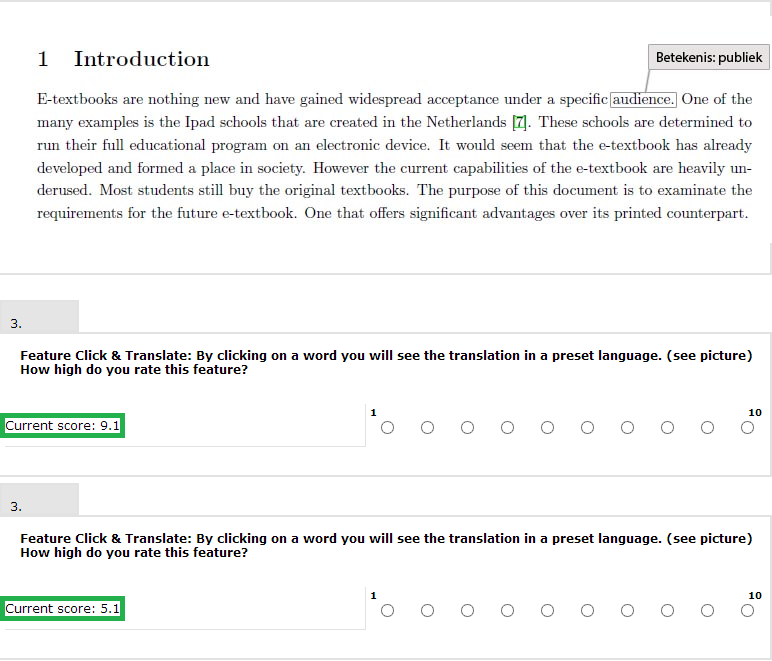
\includegraphics[width=1\textwidth]{QuestionComparison.png}
\caption{The same question, different anchoring point per questionnaire.}
\label{fig:qComp}
\end{figure}

To measure the anchoring effect we created two questionnaires, both using the same questions. While the questions are the same for both questionnaires, the averages for the questions are swapped; question `x' is rated high in one and low in the other. This setup can be seen in Figure \ref{fig:qComp}. After the experiment we measure the average and median of the participants' rating for the high and the low one to see if the anchoring had any effect on our participants.\\

If anchoring effect is real and other factors such as small experiment group don't affect the results to much than the difference between the high anchor average and the low anchor average should be positive and we should be able to observe this for a number of questions in our questionnaire.

\end{document}
